% ŠABLONA PRO PSANÍ ZÁVĚREČNÉ STUDIJNÍ PRÁCE
%%%%%%%%%%%%%%%%%%%%%%%%%%%%%%%%%%%%%%%%%%%%
% Autor: Jakub Dokulil (kubadokulil99@gmail.com)
% Tato šablona byla vytvořena tak, aby pomocí ní mohli v systému LaTeX soutěžící sázet své práce a zároveň odpovídala požadavkům na formátování vyplývajícím z wordové šablony umístěné na webu soc.cz.
%
\documentclass[12pt, a4paper,
oneside,      %% -- odkomentujte, pokud chcete svou práci mít pouze jednostrannou, mezera pro hřbet pak automaticky bude pouze na levé straně
%twoside,        %% -- pro oboustranné práce, mezera pro hřbet následně střídá strany.
openright
]{report}

%% Nutné balíčky a nastavení
%%%%%%%%%%%%%%%%%%%%%%%%%%%%

%% Proměnné
\newcommand\obor{INFORMAČNÍ TECHNOLOGIE} %% -- napiš číslo a název tvého oboru
\newcommand\kodOboru{18-20-M/01} %% -- napiš číslo a název tvého oboru
\newcommand\zamereni{se zaměřením na počítačové sítě a programování} %% -- napiš číslo a název tvého oboru
\newcommand\skola{Střední škola průmyslová a umělecká, Opava} %% vyplň název školy
\newcommand\trida{IT4} %% vyplň jméno svého konzultanta
\newcommand\jmenoAutora{Jan Stránský}  %% vyplň své jméno
\newcommand\skolniRok{2024/25} %% vyplň rok
\newcommand\datumOdevzdani{6. 1. 2025} %% vyplň rok
\newcommand\nazevPrace{CTF systém v Kubernetes} %% vyplň název své práce

\title{\nazevPrace} %% -- Název tvé práce
\author{\jmenoAutora} %% -- tvé jméno
\date{\datumOdevzdani} %% -- rok, kdy píšeš SOČku

\usepackage[top=2.5cm, bottom=2.5cm, left=3.5cm, right=1.5cm]{geometry} %% nastaví okraje, left -- vnitřní okraj, right -- vnější okraj

\usepackage[czech]{babel} %% balík babel pro sazbu v češtině
\usepackage[utf8]{inputenc} %% balíky pro kódování textu
\usepackage[T1]{fontenc}
\usepackage{cmap} %% balíček zajišťující, že vytvořené PDF bude prohledávatelné a kopírovatelné

\usepackage{graphicx} %% balík pro vkládání obrázků
\graphicspath{ {./image/} } %% cesta k obrázkům

\usepackage{subcaption} %% balíček pro vkládání podobrázků

\usepackage{hyperref} %% balíček, který v PDF vytváří odkazy

\linespread{1.25} %% řádkování
\setlength{\parskip}{0.5em} %% odsazení mezi odstavci


\usepackage[pagestyles]{titlesec} %% balíček pro úpravu stylu kapitol a sekcí
\titleformat{\chapter}[block]{\scshape\bfseries\LARGE}{\thechapter}{10pt}{\vspace{0pt}}[\vspace{-22pt}]
\titleformat{\section}[block]{\scshape\bfseries\Large}{\thesection}{10pt}{\vspace{0pt}}
\titleformat{\subsection}[block]{\bfseries\large}{\thesubsection}{10pt}{\vspace{0pt}}


\usepackage{tocloft} % Balíček umožní přizpůsobit vzhled tabulky obsahu
\setlength{\cftbeforechapskip}{0pt}  % Menší rozestup pro kapitoly
\setlength{\cftbeforesecskip}{0pt}   % Menší rozestup pro sekce

\setcounter{secnumdepth}{2}
\setcounter{tocdepth}{1}
\usepackage{fancyhdr}
\pagestyle{fancy}
\renewcommand{\headrulewidth}{0.025pt}

\usepackage{booktabs}

\usepackage{url}

%% Balíčky co se můžou hodit :) 
%%%%%%%%%%%%%%%%%%%%%%%%%%%%%%%

\usepackage{pdfpages} %% Balíček umožňující vkládat stránky z PDF souborů, 

\usepackage{upgreek} %% Balíček pro sazbu stojatých řeckých písmen, třeba u jednotky mikrometr. Například stojaté mí: \upmu, stojaté pí: \uppi

\usepackage{amsmath}    %% Balíčky amsmath a amsfonts 
\usepackage{amsfonts}   %% pro sazbu matematických symbolů
\usepackage{esint}     %% pro sazbu různých integrálů (např \oiint)
\usepackage{mathrsfs}
\usepackage{helvet} % Helvet font
\usepackage{mathptmx} % Times New Roman
\usepackage{Oswald} % Oswald font


%% makra pro sazbu matematiky
\newcommand{\dif}{\mathrm{d}} %% makro pro sazbu diferenciálu, místo toho
%% abych musel psát '\mathrm{d}' mi stačí napsat '\dif' což je mnohem 
%% kratší a mohu si tak usnadnit práci

\usepackage{listings}
\usepackage{xcolor}

\renewcommand{\lstlistingname}{Kód}% Listing -> Algorithm
\renewcommand{\lstlistlistingname}{Seznam programových kódů}% List of Listings -> List of Algorithms

%% Definice 
\lstdefinelanguage{JavaScript}{
	morekeywords=[1]{break, continue, delete, else, for, function, if, in,
		new, return, this, typeof, var, void, while, with},
	% Literals, primitive types, and reference types.
	morekeywords=[2]{false, null, true, boolean, number, undefined,
		Array, Boolean, Date, Math, Number, String, Object},
	% Built-ins.
	morekeywords=[3]{eval, parseInt, parseFloat, escape, unescape},
	sensitive,
	morecomment=[s]{/*}{*/},
	morecomment=[l]//,
	morecomment=[s]{/**}{*/}, % JavaDoc style comments
	morestring=[b]',
	morestring=[b]"
}[keywords, comments, strings]


\lstdefinelanguage[ECMAScript2015]{JavaScript}[]{JavaScript}{
	morekeywords=[1]{await, async, case, catch, class, const, default, do,
		enum, export, extends, finally, from, implements, import, instanceof,
		let, static, super, switch, throw, try},
	morestring=[b]` % Interpolation strings.
}

\lstalias[]{ES6}[ECMAScript2015]{JavaScript}

% Nastavení barev
% Requires package: color.
\definecolor{mediumgray}{rgb}{0.3, 0.4, 0.4}
\definecolor{mediumblue}{rgb}{0.0, 0.0, 0.8}
\definecolor{forestgreen}{rgb}{0.13, 0.55, 0.13}
\definecolor{darkviolet}{rgb}{0.58, 0.0, 0.83}
\definecolor{royalblue}{rgb}{0.25, 0.41, 0.88}
\definecolor{crimson}{rgb}{0.86, 0.8, 0.24}

% Nastavení pro Python
\lstdefinestyle{Python}{
	language=Python,
	backgroundcolor=\color{white},
	basicstyle=\ttfamily,
	breakatwhitespace=false,
	breaklines=false,
	captionpos=b,
	columns=fullflexible,
	commentstyle=\color{mediumgray}\upshape,
	emph={},
	emphstyle=\color{crimson},
	extendedchars=true,  % requires inputenc
	fontadjust=true,
	frame=single,
	identifierstyle=\color{black},
	keepspaces=true,
	keywordstyle=\color{mediumblue},
	keywordstyle={[2]\color{darkviolet}},
	keywordstyle={[3]\color{royalblue}},
	literate=%
	{á}{{\'a}}1 {č}{{\v{c}}}1 {ď}{{\v{d}}}1 {é}{{\'e}}1 {ě}{{\v{e}}}1
	{í}{{\'i}}1 {ň}{{\v{n}}}1 {ó}{{\'o}}1 {ř}{{\v{r}}}1 {š}{{\v{s}}}1
	{ť}{{\v{t}}}1 {ú}{{\'u}}1 {ů}{{\r{u}}}1 {ý}{{\'y}}1 {ž}{{\v{z}}}1,		
	numbers=left,
	numbersep=5pt,
	numberstyle=\tiny\color{black},
	rulecolor=\color{black},
	showlines=true,
	showspaces=false,
	showstringspaces=false,
	showtabs=false,
	stringstyle=\color{forestgreen},
	tabsize=2,
	title=\lstname,
	upquote=true  % requires textcomp	
}


\lstdefinestyle{JSES6Base}{
	backgroundcolor=\color{white},
	basicstyle=\ttfamily,
	breakatwhitespace=false,
	breaklines=false,
	captionpos=b,
	columns=fullflexible,
	commentstyle=\color{mediumgray}\upshape,
	emph={},
	emphstyle=\color{crimson},
	extendedchars=true,  % requires inputenc
	fontadjust=true,
	frame=single,
	identifierstyle=\color{black},
	keepspaces=true,
	keywordstyle=\color{mediumblue},
	keywordstyle={[2]\color{darkviolet}},
	keywordstyle={[3]\color{royalblue}},
 literate=%
{á}{{\'a}}1 {č}{{\v{c}}}1 {ď}{{\v{d}}}1 {é}{{\'e}}1 {ě}{{\v{e}}}1
{í}{{\'i}}1 {ň}{{\v{n}}}1 {ó}{{\'o}}1 {ř}{{\v{r}}}1 {š}{{\v{s}}}1
{ť}{{\v{t}}}1 {ú}{{\'u}}1 {ů}{{\r{u}}}1 {ý}{{\'y}}1 {ž}{{\v{z}}}1,		
	numbers=left,
	numbersep=5pt,
	numberstyle=\tiny\color{black},
	rulecolor=\color{black},
	showlines=true,
	showspaces=false,
	showstringspaces=false,
	showtabs=false,
	stringstyle=\color{forestgreen},
	tabsize=2,
	title=\lstname,
	upquote=true  % requires textcomp
}

\lstdefinestyle{JavaScript}{
	language=JavaScript,
	style=JSES6Base,
}
\lstdefinestyle{ES6}{
	language=ES6,
	style=JSES6Base
}


%% Bordel pro práci - můžeš smáznout :) 
%%%%%%%%%%%%%%%%%%%

\usepackage{lipsum} %% balíček který píše lipsum (nesmyslný text, který se používá pro kontrolu typografie)

%% Začátek dokumentu
%%%%%%%%%%%%%%%%%%%%
\begin{document}
	
	\pagestyle{empty}
	\pagenumbering{Roman}
	
	\cleardoublepage

%% Titulní stránka s informacemi
%%%%%%%%%%%%%%%%%%%%%%%%%%%%%%%%%%%%%%%%
	
	{\fontfamily{phv}\selectfont
		%% Logo školy
		\begin{figure}[h]
			\centering
			
\includegraphics[width=0.6\linewidth]{image/logo-skoly.png} 
		\end{figure}
		
		
		%% Hlavička práce a její název (viz proměnná \nazev prace)
		%% \sffamily %%% bezpatkové písmo - sans serif
		{\bfseries %%% písmo na stránce je tučně
			\begin{center}
				\vspace{0.025 \textheight}
				\LARGE{ZÁVĚREČNÁ STUDIJNÍ PRÁCE}\\
				\large{dokumentace}\\
				\vspace{0.075 \textheight}
				\LARGE {\nazevPrace}\\
			\end{center}  
		}%%%
		
		%\begin{figure}[h]
			%\centering
			%
\includegraphics[width=0.8\linewidth]{image/programovani-02.jpg} 
		%\end{figure}
		
		\vspace{0.02 \textheight}
		\begin{table}[h!]
			\begin{tabular}{ll}
				\textbf{Autor:} & \jmenoAutora\\ 
				\textbf{Obor:} & \kodOboru { } \obor\\
				\textbf{} & \zamereni\\
				\textbf{Třída:} & \trida\\
				\textbf{Školní rok:} & \skolniRok\\
			\end{tabular}
			
		\end{table}		
	}
	
\cleardoublepage %% Zalomení dvojstránky
	
%% Stránka obsahující poděkování a prohlášení
%%%%%%%%%%%%%%%%%%%%%%%%%%%%%%%%%%%%%%%%%%%%%%%%%%%%%%%%

%% Poděkování - nepovinné
%%%%%%%%%%%%%%%%%%%%%%%%%%%%
	
	\noindent{\large{\bfseries{Poděkování}\\}}
	\noindent Rád bych poděkoval pánům učitelům Ing. Petru Grussmannovi a Mgr. Marku Lučnému za jejich pomoc s projektem, jelikož mi poskytovali cenné rady a připomínky.

	
	\vspace*{0.7\textheight} %% Vertikální mezeru je možné upravit

%% Prohlášení - povinné
%%%%%%%%%%%%%%%%%%%%%%%%%%%%
	\noindent{\large{\bfseries{Prohlášení}\\}}  %% uprav si koncovky podle toho na jaký rod se cítíš, vypadá to pak lépe :) 
	\noindent{Prohlašuji, že jsem závěrečnou práci vypracoval samostatně a uvedl veškeré použité 
		informační zdroje.\\}
	\noindent{Souhlasím, aby tato studijní práce byla použita k výukovým a prezentačním účelům na Střední průmyslové a umělecké škole v Opavě, Praskova 399/8.}
	\vfill
	\noindent{V Opavě \datumOdevzdani\\}
	\noindent
	\begin{minipage}{\linewidth}
		\hspace{9.5cm} 
		\begin{tabular}{@{}p{6cm}@{}}
			\dotfill \\
			Podpis autora
		\end{tabular}
	\end{minipage}
	
	\cleardoublepage %% Zalomení dvojstránky

%% Stránka obsahující abstrakt (anotaci)
%%%%%%%%%%%%%%%%%%%%%%%%%%%%%%%%%%%%%%%%%%%%%%%%%%%%%%%%	

%% Abstrakt v češtině
%%%%%%%%%%%%%%%%%%%%%%%%%%%%
	\noindent{\Large{\bfseries{Abstrakt}\\}}
	\noindent Výsledkem tohoto projektu je funkční systém pro spouštění a vytváření úloh CTF typu v systému Kubernetes běžícím na školní síti s dostatečnou mírou zabezpečení. Aplikace zahrnuje registraci a přihlašování uživatelů, zapínání nových úloh a následně jejich vypínání. Hlavní částí tohoto projektu je komunikace se systémem Kubernetes, který se využívá ve vysoce škálovaných produkčních prostředích. Uživatel s aplikací může komunikovat skrz poskytnuté webové prostředí, ale může komunikovat i přímo s poskytnutou API. Dále si tento projekt klade za cíl umožnit studentům se lépe seznámit s určitými možnostmi v oblasti IT formou hry (CTF) jako to dělají služby jako např. TryHackMe nebo HackTheBox.
	
	\vspace{18pt}
	
	\noindent{\large{\bfseries{Klíčová slova}}}
	
	\noindent CTF, Kubernetes, FastAPI, webová aplikace
	
	\vspace{18pt}

%% Abstrakt v angličtině
%%%%%%%%%%%%%%%%%%%%%%%%%%%%	
	\noindent{\Large{\bfseries{Abstract}}}
	
	\noindent The result of this project is a functional system for running and creating CTF type tasks in the Kubernetes system running on the school network with a sufficient level of security. The application includes user registration and login, turning on new tasks and then turning them off. The main part of this project is communication with the Kubernetes system, which is used in highly scalable production environments. The user can communicate with the application through the provided web interface, but can also communicate directly with the provided API. Furthermore, this project aims to allow students to better familiarize themselves with certain IT options through a game (CTF) like services TryHackMe or HackTheBox do.

	
	\vspace{18pt}
	
	\noindent{\large{\bfseries{Keywords}}}
	
	\noindent CTF, Kubernetes, FastAPI, web application	
	\clearpage %% Zalomení stránky

%% Stránka s generovaným obsahem
%%%%%%%%%%%%%%%%%%%%%%%%%%%%%%%%%%%%%%%	
	
	\tableofcontents %% Vygeneruje tabulku s obsahem

	\pagenumbering{arabic} %% Nastavení způsobu číslování stránek (alternativy roman | Roman)
	\setcounter{page}{1} %% Nastavení počitadla stránek

%% Stránka s úvodem - povinná část
%%%%%%%%%%%%%%%%%%%%%%%%%%%%%%%%%%%%%%%		
	\chapter*{Úvod}
%Tento příkaz vytvoří novou kapitolu s názvem "Úvod" ve vašem dokumentu.
%Hvězdička * u příkazu \chapter* znamená, že tato kapitola nebude mít číslo. Ve výsledném dokumentu se tedy objeví jako "Úvod" bez předcházejícího čísla kapitoly, které se obvykle zobrazuje u číslovaných kapitol.
%Tento příkaz také znamená, že kapitola se automaticky neobjeví v obsahu, protože LaTeX standardně zahrnuje do obsahu pouze číslované kapitoly.
	\addcontentsline{toc}{chapter}{Úvod}
%Tento příkaz ručně přidává záznam do obsahu.
%První parametr toc označuje, že přidáváme záznam do Table of Contents (obsahu).
%Druhý parametr chapter specifikuje úroveň záznamu. V tomto případě říkáme, že přidávaný záznam má být považován za kapitolu.
%Třetí parametr Úvod je text, který se objeví v obsahu. V tomto případě bude v obsahu zobrazen název "Úvod".	

Mým cílem v této práci bylo sestavit škálovatelný software, který by nad prostředím Kubernetes vytvářet a spravovat kontejnery pro soutěž typu CTF (Capture The Flag). Zároveň bylo cílem, aby se tento software dal nasadit i v prostředí s nízkým oprávněním a aby ho šlo škálovat díky architektuře mikroslužeb.

Hlavní motivací bylo pochopení funkce a komunikace v rámci aplikací s formátem typu mikroslužeb místo monolitických aplikací a zlepšení svých dovedností v oblasti prostředí Kubernetes.

Zvláštní zaměření bylo na backendovou část API a na zabezpečení celého systému.

\chapter{Problematika efektivního hostovaní CTF systému}
CTF (Capture The Flag) je forma soutěže a interaktivního vzdělávání, kde se účastníci snaží získat co nejvíce vlajek (flag) z různých úloh. Obvykle se jedná o úlohy z oblasti kybernetické bezpečnosti, ale mohou být i z jiných oblastí jako např. programování, matematika, atd. Já jsem se ve svém projektu rozhodl zkusit vytvořit funkční CTF systém spustitelný na školní instanci Kubernetes. 

Obvykle se při tvorbě takových systémů brzy narazí na problémy s bezpečností samotného systému vzhledem k tomu, že se jedná o systém, který musí mít alespoň omezený přístup k jinému systému kde může spouštět kontejnery, tím pádem musí zajistit, že tento systém nelze v případě úspěšného útoku na administrátorský účet zneužít na eskalaci práv na samotný hostitelský cluster. Toto je obvykle zajištěno využitím již existujících cloudových hosting platforem (např. Amazon AWS EC2), ale v tomto projektu jsem se rozhodl pokusit o řešení tzv. on-prem nasazení, kde tento kód využívá čistě již vytvořených zdrojů bez automatického provizování nových od cloudového poskytovatele, což znatelně zvyšuje komplexitu celého systému, ale zároveň snižuje riziko nečekaných nákladů kvůli opomenutým cloudovým strojům, které jsou obvykle placeny nejen za minutu provozu, ale i za přenos dat, což se může u některých typů úloh stát velmi drahým kvůli množství paketů, které se musí přenést. 

Avšak, on-prem řešení má problémy s určitými požadavky - např. může být problém zajistit přístup ke kontejnerům, který je jinak obvykle řešen buď přímým přístupem přes přiřazenou IP adresu, VPN nebo přes službou poskytnutý "Attack Box," což je samostatný kontejner s nástroji pro účastníky, který je připojen k interní síti a může být použit pro útoky na úlohy. Přístup k tomuto boxu je obvykle řešen přes webový prohlížeč. Dalším problémem je zabezpečení samotného systému, kde je nutné zajistit, aby účastníci nemohli získat přístup k jiným účastníkům nebo k samotnému hostitelskému systému. 

\section{Využití v praxi}
Nejčastěji se CTF systémy využívají pro vzdělávání a trénování v oblasti kybernetické bezpečnosti, kde se účastníci snaží získat co nejvíce vlajek (flag) z různých úloh. Toto je obvykle prováděno v rámci škol nebo na veřejných soutěžích, kde se účastníci snaží získat co nejvíce bodů za úspěšné řešení úloh, čímž lze přitáhnout nové talenty do oblasti kybernetické bezpečnosti. Zároveň jsou CTF soutěže ideální formou vzdělávání hrou, jelikož účastníci se učí nové věci formou hry, což je obvykle mnohem efektivnější než tradiční vzdělávání.

Zároveň tyto platformy umožňují jednoduše vytvářet nové úlohy a zároveň je možné je jednoduše škálovat, což je důležité pro velké soutěže, kde se může zúčastnit až několik tisíc účastníků. Toto je zajištěno samotnou architekturou těchto platforem, které v případě on-prem řešení nejčastěji využívají Kubernetes nebo jeho nadstavbou jako je třeba OpenShift od společnosti RedHat.

\section{Cíle práce}
Jak již bylo zmíněno v úvodu, cílem této práce bylo vytvořit funkční CTF systém spustitelný na školní instanci Kubernetes, který by byl schopen spouštět a vytvářet úlohy pro soutěže typu CTF. Zároveň bylo cílem, aby se tento software dal nasadit i v prostředí s nízkým oprávněním a aby ho šlo škálovat díky architektuře mikroslužeb. V rámci tohoto projektu jsem se rozhodl využít technologie jako FastAPI, Kubernetes a SQLAlchemy, které mi umožnily vytvořit funkční systém, který by byl schopen spouštět a vytvářet úlohy pro soutěže typu CTF. 

Důležitým cílem bylo také zabezpečení celého systému, aby nedošlo k úniku dat nebo k zneužití systému k útokům na jiné účastníky nebo na samotný hostitelský systém, což bylo zajištěno využitím schopnosti mikroslužeb v tom, že každá část má přístup pouze k tomu, co potřebuje a nemá přístup k ostatním částem systému, což je důležité např. u JWT klíče, kde všechny části systému potřebují přístup k veřejnému klíči, ale k privátnímu klíči má přistup pouze služba Auth. Toto je také důvod využití algoritmu RS256 (asymetrického šifrování) místo běžnějšího algoritmu HS256 (symetrického šifrování), kde by měly všechny části přístup ke klíči, který umožňuje podepisovat JWT tokeny.

%Tipy k psaní úvodu
%Je povinný, nadpis neměňte, rozsah - max. 1 strana. 
%Tato část práce obsahuje: 
%* náhled do řešené problematiky, zdůvodnění volby problematiky, 
%* předem definované cíle práce, 
%* motivaci pro další čtení textu včetně stručného uvedení obsahu následujících kapitol 

\chapter{Využité technologie}

\section{Backend}

\subsection{Kubernetes}
Tento projekt využíval na zprovoznění a správu samotných úloh Kubernetes. Kubernetes je open-source platforma pro orchestraci kontejnerů, která umožňuje automatizovat nasazování, škálování a správu aplikací běžících v kontejnerech. 

Tato platforma má zároveň plnohodnotnou REST API a oficiální knihovnu pro jazyk Python, což např. systém Docker standardně neobsahuje. Zároveň má možnost vzdálené správy, díky čemuž se daly samotné mikroslužby jednoduše restartovat a aktualizovat bez nutnosti přímého přístupu na server pomocí SSH nebo webového rozhraní (např. Portainer). Toto mi později pomohlo při debugování a vývoji.

Tento systém se dá v případě potřeby škálovat a to jak na lokálních serverech, tak také na cloudu v případě, že by bylo potřeba zvýšit výkon nebo dostupnost systému.

Abych nemusel vytvářet nový systém, tak jsem se rozhodl využít Kubernetes, který běží na školní síti a je dostupný pro všechny studenty.

\subsubsection{vCluster}
Vzhledem k požadavku, aby byl systém spustitelný na školní instanci Kubernetes, jsem se rozhodl využít Kubernetes vcluster, který je dostupný pro všechny studenty a zároveň je možné vytvářet nové namespace a pody, čímž se dají mnohem jednodušeji zařizovat případná práva přes RBAC systém ke kterému žáci standardně přístup nemají.

VCluster je program, který umožňuje vytvářet virtuální clustery na již běžícím Kubernetes clusteru, čímž umožňuje získat uživateli "zvýšená" práva oproti standardnímu clusteru. Tento program mi umožnil vytvořit vlastní cluster, který byl dostupný pouze mně a zároveň mi umožnil vytvářet nové namespace a pody, což bylo důležité pro zajištění bezpečnosti a izolace jednotlivých úloh jelikož bezpečnostní arvhitektura tohoto systému očekává, že uživatelské úlohy běží na jiném clusteru než samotný systém.

\subsection{FastAPI}
FastAPI je moderní webový framework napsaný v jazyce Python, který je založen na standardu ASGI (Asynchronous Server Gateway Interface). Tento framework je velmi rychlý a zároveň je velmi jednoduchý na použití a má velmi dobrou dokumentaci. Díky tomu jsem se rozhodl použít tento framework pro vytvoření API části tohoto projektu.

Tento framework mi jednoduše umožnil psát API backend v jazyce Python a zároveň mi umožnil využívat asynchronní programování, což bylo důležité pro rychlou odezvu API.

Zároveň mi tento framework velmi zjednodušil zajištění čitelnosti kódu díky vynucenému využití typování a automatickému generování dokumentace.

\subsection{SQLAlchemy}
SQLAlchemy je knihovna pro jazyk Python, která umožňuje komunikaci s relačními databázemi pomocí SQL. Tato knihovna mi umožnila vytvořit ORM (Object-Relational Mapping) pro databázi PostgreSQL, díky čemuž jsem mohl jednoduše vytvářet a upravovat databázové tabulky pomocí Pythonu bez nutnosti psát SQL dotazy a kontrolovat bezpečnost uživatelských vstupů.

\subsection{Redis}
Na uchování již nastartovaných úloh jsem použil databázi Redis. Redis je open-source in-memory databáze, která je používána pro ukládání klíč-hodnota párů. Tato databáze mi umožnila ukládat informace o běžících úlohách a zároveň mi umožnila jednoduše získávat informace o těchto úlohách.

Redis se standardně využívá např. na ukládání cache, ale v tomto projektu jsem ho využil na ukládání informací o běžících úlohách, jelikož je velmi rychlý a jednoduchý na použití.

\subsection{Databáze}
Jakožto databázi jsem zvolil PostgreSQL, která je open-source relační databáze. Tato databáze mi umožnila ukládat informace o uživatelích, úlohách a dalších informacích, které byly potřeba pro správné fungování tohoto projektu. 

Tuto databázi jsem zvolil z důvodu, že je velmi rychlá, je velmi dobře podporována knihovnou SQLAlchemy a je vhodná pro produkční nasazení.

\subsection{JWT}
Na autentizaci jsem použil JWT (JSON Web Token), který mi umožnil vytvářet a ověřovat tokeny, které byly použity pro ověření uživatele v ostatních částech systému. Tento token byl podepsán pomocí privátního klíče (algoritmus RSA) a ověřován pomocí veřejného klíče. Tyto tokeny byly ukládány do cookie a zároveň byly přenášeny v hlavičce požadavku.

Tento algoritmus mi umožnil zajištění bezpečnosti uživatelů a zároveň mi umožnil jednoduché ověřování uživatelů v ostatních částech systému díky jeho bezestavové povaze.

Samotné klíče jsem ukládal do Kubernetes Secret, což mi umožnilo jednoduše měnit klíče na jednom místě bez nutnosti změn v samotných aplikacích.


\section{Frontend}
\subsection{React}
Na frontend jsem využil toolkit Vite a knihovnu React. React je knihovna pro tvorbu uživatelských rozhraní, která je vyvíjena a udržována společností Facebook. Tato knihovna mi umožnila vytvořit jednoduché a rychlé webové rozhraní, které bylo zároveň jednoduché na údržbu a rozšíření.

Využití Reactu mi umožnilo zajištění rychlé odezvy a zároveň jednoduchého vytváření komponent, což mi zjednodušilo vytváření webového rozhraní vzhledem k tomu, že frontend nebyl primární částí tohoto projektu.

Na kód jsem využil JavaScript jelikož jsem s ním již měl zkušenosti, které jsem postrádal u TypeScriptu.

\section{Ostatní části}
\subsection{Git submodules}
Pro sdílení modelů mezi mikroslužbami jsem využil Git Submodules, které mi umožnily sdílet kód mezi jednotlivými mikroslužbami a zároveň mi umožnily jednoduše aktualizovat kód v jednotlivých mikroslužbách bez nutnosti hlídat aktuálnost zkopírovaného kódu.

Toto mi navíc umožnilo jednoduše sdílet kód mezi jednotlivými částmi systému a zároveň mi umožnilo jednoduše měnit kód v jednotlivých částech systému.


\chapter{Řešení backendu - mikroslužby}

\section{Úvod}
\label{sec:uvod}

V této kapitole se seznámíme s tím, co mikroslužby jsou a s jednotlivými mikroslužbami použitými v API částí tohoto projektu. Všechny tyto mikroslužby jsou napsány v jazyce Python s použitím 

Na autentizace byly použity JWT tokeny, které byly podepsány pomocí privátního klíče (algoritmus RSA) a ověřovány pomocí veřejného klíče. Tyto tokeny byly ukládány do cookie a zároveň byly přenášeny v hlavičce požadavku.

Tyto mikroslužby jsou:
\begin{itemize}
	\item Router
	\item Auth
	\item Lister
	\item Deployer 
	\item Deleter
	\item Flag-submitter
\end{itemize}

\section{Router}
Tato mikroslužba je zodpovědná za směrování požadavků na správné mikroslužby a veškeré požadavky na API putují skrz ni, díky čemuž se dá využít globální modifikace, monitorování a logování požadavků. Kvůli tomuto účelu tato služba nepotřebuje žádné privilegované přístupy do ostatních částí systému. Jednou z částí této mikroslužby je i zajištění přesunu JWT tokenu z cookie do hlavičky požadavku, aby se dala API používat jak z webového frontendu, tak i z jiných aplikací.

Tato mikroslužba zároveň funguje jakožto filtr nevalidních typů požadavků (dále posílá pouze požadavky typu GET, POST, PUT a DELETE, ostatní jsou zahozeny s chybovou hláškou)

\section{Auth}
Tato mikroslužba je zodpovědná za registraci uživatele a vytvářením jeho záznamu v databázi PostgreSQL. 

Tato služba je jediná, která má přístup k privátnímu klíči použivaného k podepisování tokenů algoritmem RS256. Dále je také zodpovědná za ověření přihlašovacích údajů uživatele a vytvoření JWT tokenu, který se následně používá pro ověření uživatele v ostatních částech systému. Tato služba má přístup k databázi PostgreSQL.

Tato služba má tři API endpointy:
\begin{itemize}
	\item POST /register
	\item POST /login
	\item GET /health
\end{itemize}
kde první dva slouží k registraci a přihlášení uživatele a třetí slouží k zjištění stavu služby, primárně kvůli liveness a readiness HTTP checku v Kubernetes při chybě nebo při čekání na databázi.

\section{Lister}
Účel mikroslužby Lister je umožnění uživatelům získat informace o všech dostupných úlohách a jejich stavech. Dále tato služba umožňuje získat data o právě aktivních úlohách uživatele a získání detailních informací o těchto úlohách.

Tato mikroslužba potřebuje přístup k Redis a PostgreSQL databázím.

Tato služba má čtyři API endpointy:
\begin{itemize}
	\item GET /
	\item GET /running
	\item GET /running/{id}
	\item GET /health
\end{itemize}
kde první endpoint vrací veškeré dostupné úlohy a nepotřebuje žádné přihlášení, zatímco druhý a třetí endpoint vrací informace o právě běžících úkolech uživatele, tudíž vyžadují token, s tím, že třetí vrací i detailní informace o tomto úkolu.

\section{Deployer}
Tato mikroslužba zajišťuje zapínání úkolů uživatele v systému Kubernetes a zapsání informací o této běžící službě do databáze Redis, čímž zpřístupní tato data službě Lister.

Jednotlivé úkoly jsou v Kubernetes spuštěné jakožto pody v namespace daným uživatelem, což je také jeden z důvodů užívání samostatného Kubernetes clusteru (ať už opravdového nebo vcluster) pro tyto studentské stroje - ServiceAccount  spojený s tímto projektem musí mít jak práva na vytváření nových podů, tak vytváření nových namespace.

Tato služba vyžaduje přístup k Redis a PostgreSQL databázím a ke Kubernetes API.

Tato služba má dva API endpointy:
\begin{itemize}
	\item POST /
	\item GET /health
\end{itemize}
kde základní endpoint vyžaduje JSON data s \texttt{challenge\_id} klíčem. Dále tento endpoint potřebuje přístup k tokenu.

\begin{lstlisting}[style=Python, caption=Ukázka kódu pro vytvoření instance]
@app.post("/")
def create_instance(x_token: Annotated[str, Header()], data: Data):
    print(f"creating instance {data}")
    payload = None
    try:
        with open(PUBLIC_KEY_PATH, 'r') as f:
            public_key = f.read()
            payload = decode(x_token, public_key, algorithms=['RS256'])
    except Exception as e:
        raise HTTPException(status_code=401, detail="Invalid token")
    user_id = payload["sub"]
    image_id = data.challenge_id
    print(kube.create_in_k8s(db=db, 
			     user_id=user_id, 
			     challenge_id=image_id))
    print("Redis")
    r.create_instance(user_id=user_id, image_id=image_id)
    return {"status": "success"}
\end{lstlisting}

\section{Deleter}
Tato mikroslužba umožňuje vypínat (mazat) již vytvořené úkoly uživatele a to jak v Redis databázi, tak jejich instance běžící v systému Kubernetes.

Tato služba vyžaduje přístup k Redis databázi a ke Kubernetes API.

Tato služba má dva API endpointy:
\begin{itemize}
	\item DELETE /{id}
	\item GET /health
\end{itemize}
kde endpoint \texttt{/\{id\}} vyžaduje id úkolu, který uživatel chce vypnout a JWT token uživatele.

\section{Flag-submitter}
Tato mikroslužba umožňuje odevzdávat řešení jednotlivých úkolů (vlajky).

Tato služba vyžaduje přístup k PostgreSQL databázi.

Tato služba má dva API endpointy:
\begin{itemize}
	\item POST /{flag\_id}
	\item GET /health
\end{itemize}
kde endpoint \texttt{/\{flag\_id\}} vyžaduje v těle požadavku string \texttt{flag} a token uživatele.

\section{Přístup k systémům}
Kvůli nastazení jsem se rozhodl pro připojování k databázím a ke Kubernetesu na backendu používat na míru vytvořené třídy, které mi umožnily připojit se k těmto systémům a využívat funkce pro komunikaci s nimi bez nutnosti se obtěžovat s vytvářením nových připojení a zároveň mi umožnilo jednoduše měnit přístupové údaje k těmto systémům.

\begin{lstlisting}[style=Python, caption=Ukázka třídy pro připojení ke Kubernetes]
from kubernetes import client, config
from kubernetes.utils import create_from_dict

class Kubernetes:
    def __init__(self, key, url):
        self.configuration = client.Configuration()
        self.configuration.api_key['authorization'] = key
        self.configuration.api_key_prefix['authorization'] = 'Bearer'
        self.configuration.host = url
        self.configuration.verify_ssl = False
        self.client = client.ApiClient(self.configuration)
        self.v1 = client.CoreV1Api(self.client)
    def get_k8s_config(self):
        return self.v1
    def create_namespace(self, name: str):
        body = client.V1Namespace(metadata=client.V1ObjectMeta(name=name))
        return self.v1.create_namespace(body)

    def namespace_exists(self, name: str):
        namespaces = self.v1.list_namespace()
        for ns in namespaces.items:
            if ns.metadata.name == name:
                return True
        return False
	...
\end{lstlisting}

\chapter{Frontend}
Frontend část tohoto projektu je napsána v Reactu a jakožto nástroje je využíván projekt Vite. Samotná stránka funguje na bázi CSR (Client Side Rendering) a komunikuje s API popsáným v předchozí kapitole. Díky tomuto je tato stránka zároveň kódově oddělená od backendové části a může být nasazena na jiném serveru než backend a může být psána v jiném jazyce než backendová část. Frontend je napsán v JavaScriptu díky jeho jednoduchosti a rychlosti vývoje.

První stránka, kterou člověk vidí, je přihlašovací formulář a navigační lišta. Po přihlášení se zobrazí stránka s úlohami, které může uživatel zapínat a vypínat. Dále je zde možnost zobrazit si informace o právě běžících úlohách a o všech dostupných úlohách.

Využití Reactu umožňuje stránce být tzv. SPA (Single Page Application) a tím pádem se nemusí stránka znovu načítat při každém přechodu mezi stránkami, což zvyšuje rychlost a plynulost stránky. Zároveň díky tomuto přístupu může webový server frontendu pouze posílat statické soubory a nemusí se starat o žádnou logiku, což zvyšuje bezpečnost a snižuje nároky na server.

\begin{figure}[h]
	\centering
	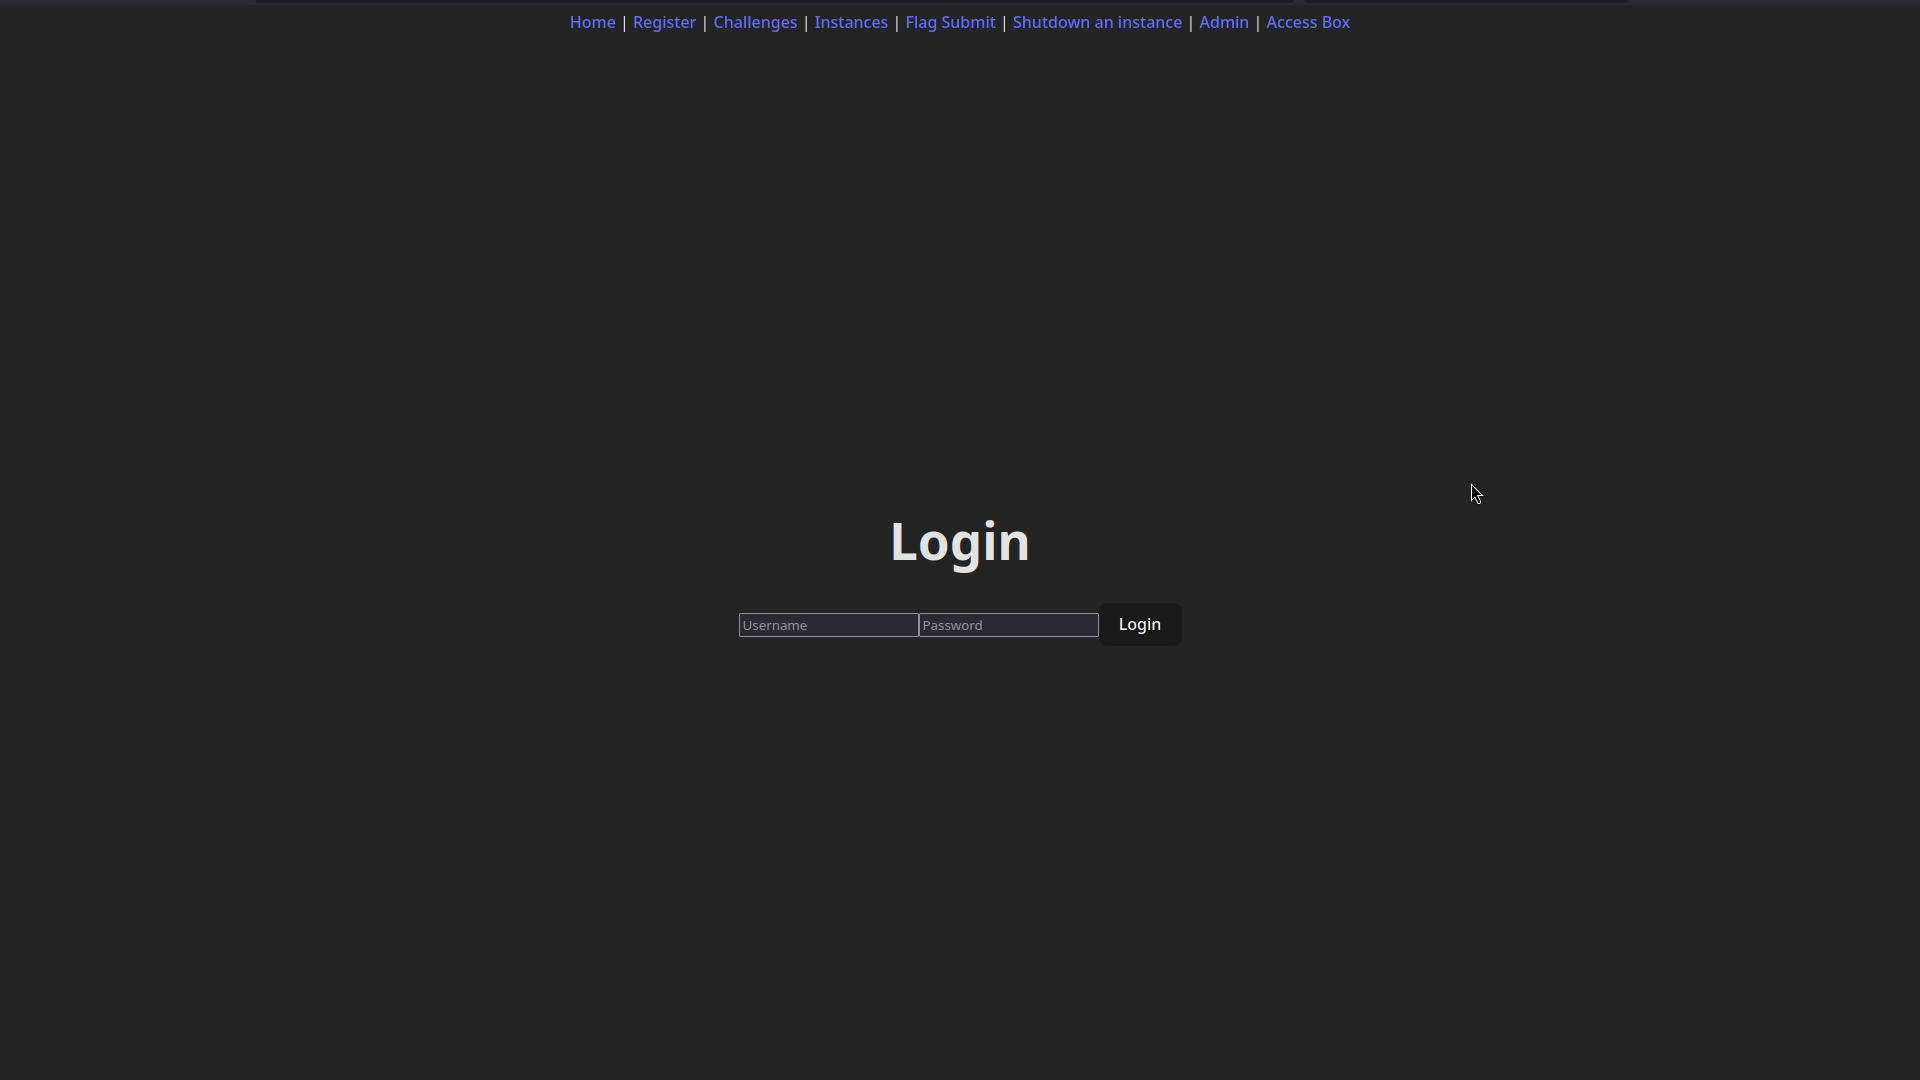
\includegraphics[width=0.8\textwidth]{01-login_screen.png}
	\caption{Přihlašovací formulář}
	\label{fig:frontend-login}
\end{figure}

\section{Challenges}
Na této stránce je možné vidět všechny dostupné úlohy a zároveň je možné tyto úlohy zapínat. U každé z těchto úloh je poskytnuto ID úlohy a její název. Po kliknutí na tlačítko "Deploy" se úloha zapne a zobrazí se v sekci "Instances".

\begin{figure}[h]
	\centering
	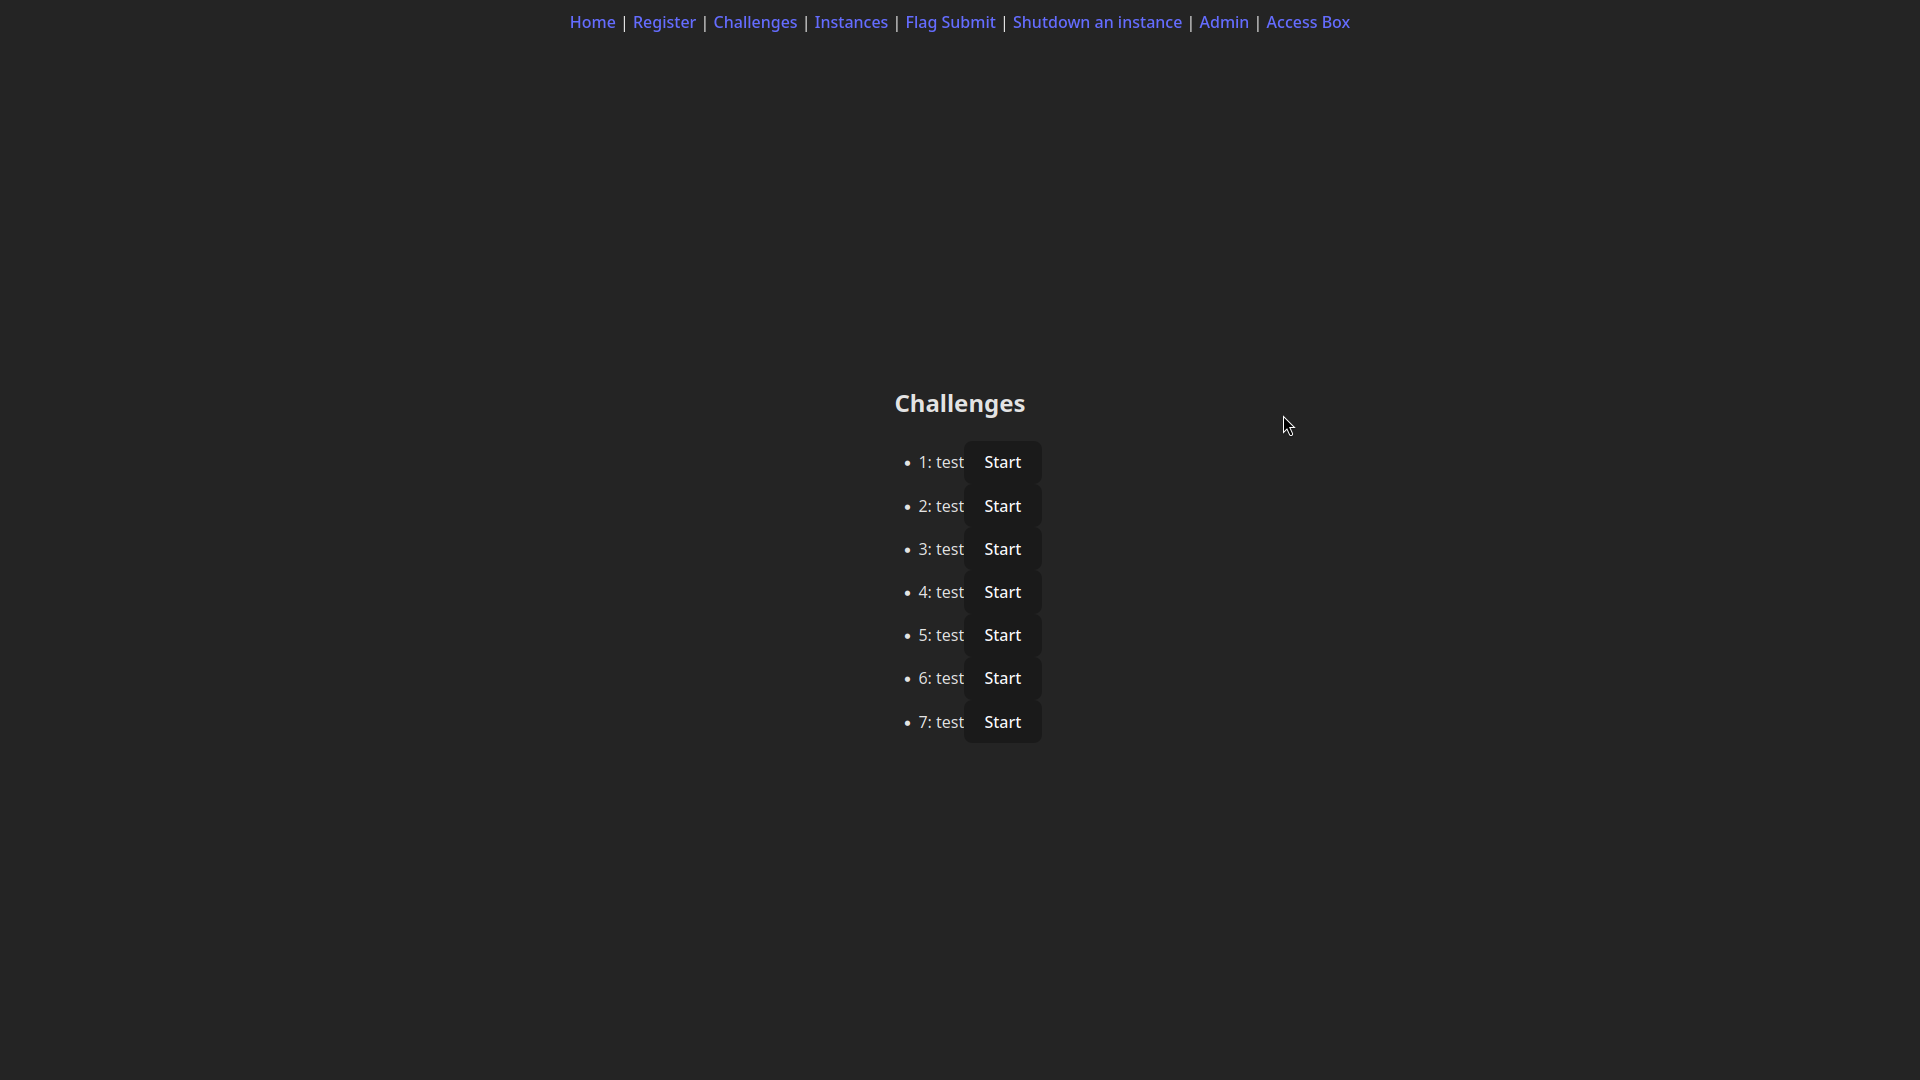
\includegraphics[width=0.8\textwidth]{02-challenges.png}
	\caption{Seznam úloh}
	\label{fig:frontend-challenges}
\end{figure}

\begin{figure}[h]
	\centering
	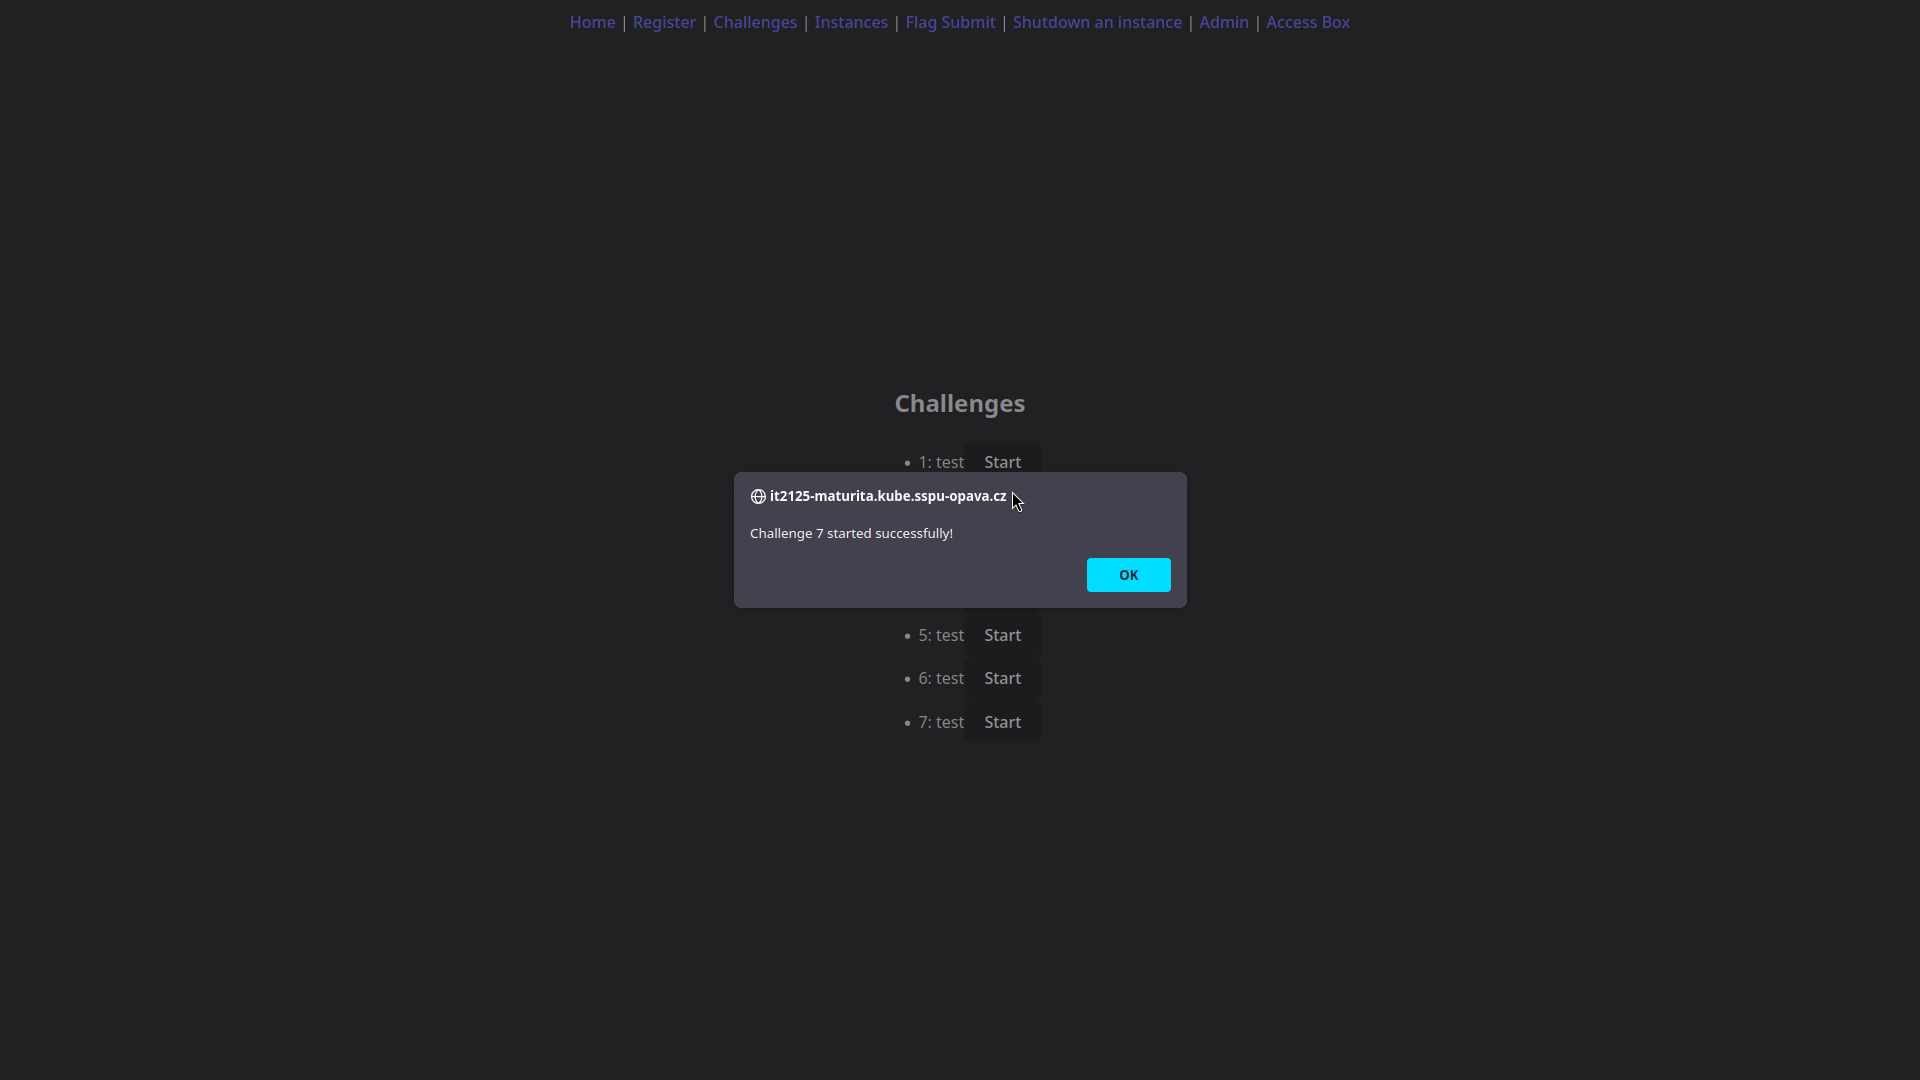
\includegraphics[width=0.8\textwidth]{03-challenges_success.png}
	\caption{Úloha úspěšně zapnuta}
	\label{fig:frontend-challenges-success}
\end{figure}

\section{Instances}
Na této stránce je možné vidět všechny právě běžící úlohy uživatele a zároveň je možné tyto úlohy vypínat. U každé z těchto úloh je poskytnuto ID úlohy.

%\begin{figure}[h]
	%\centering
	%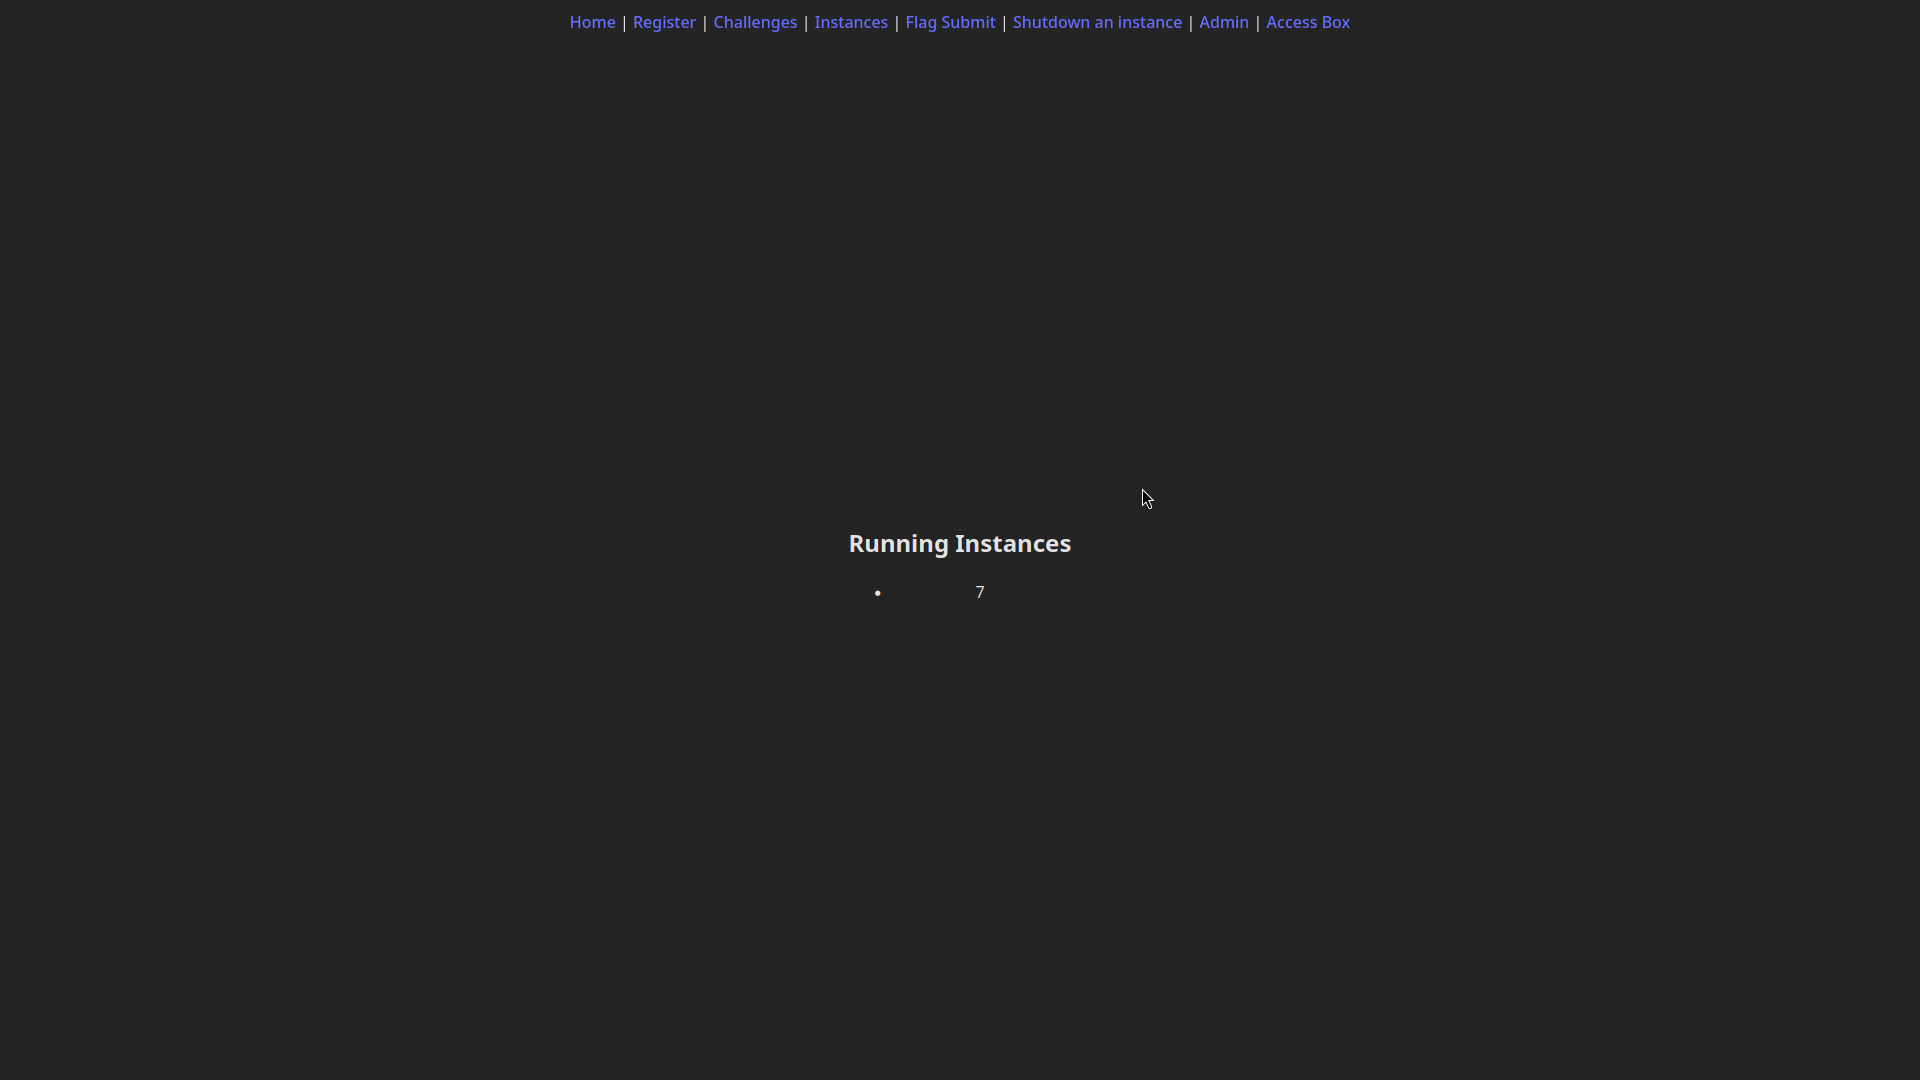
\includegraphics[width=0.8\textwidth]{04-instances.png}
	%\caption{Seznam běžících úloh}
	%\label{fig:frontend-instances}
%\end{figure}

\section{Flag submit}
Na této stránce je možné odevzdávat vlajky k jednotlivým úlohám. Po odevzdání vlajky se zobrazí zpráva, zda byla vlajka správná nebo ne. Tento přístup k odevzdávání vlajek má své výhody, ale i své problémy - výhodou je, že uživatel může pracovat na více úlohách najednou bez hledání k jaké části vlajka patří, ale zároveň to znemožňuje mít jednu vlajku na více úlohách.

\begin{figure}[h]
	\centering
	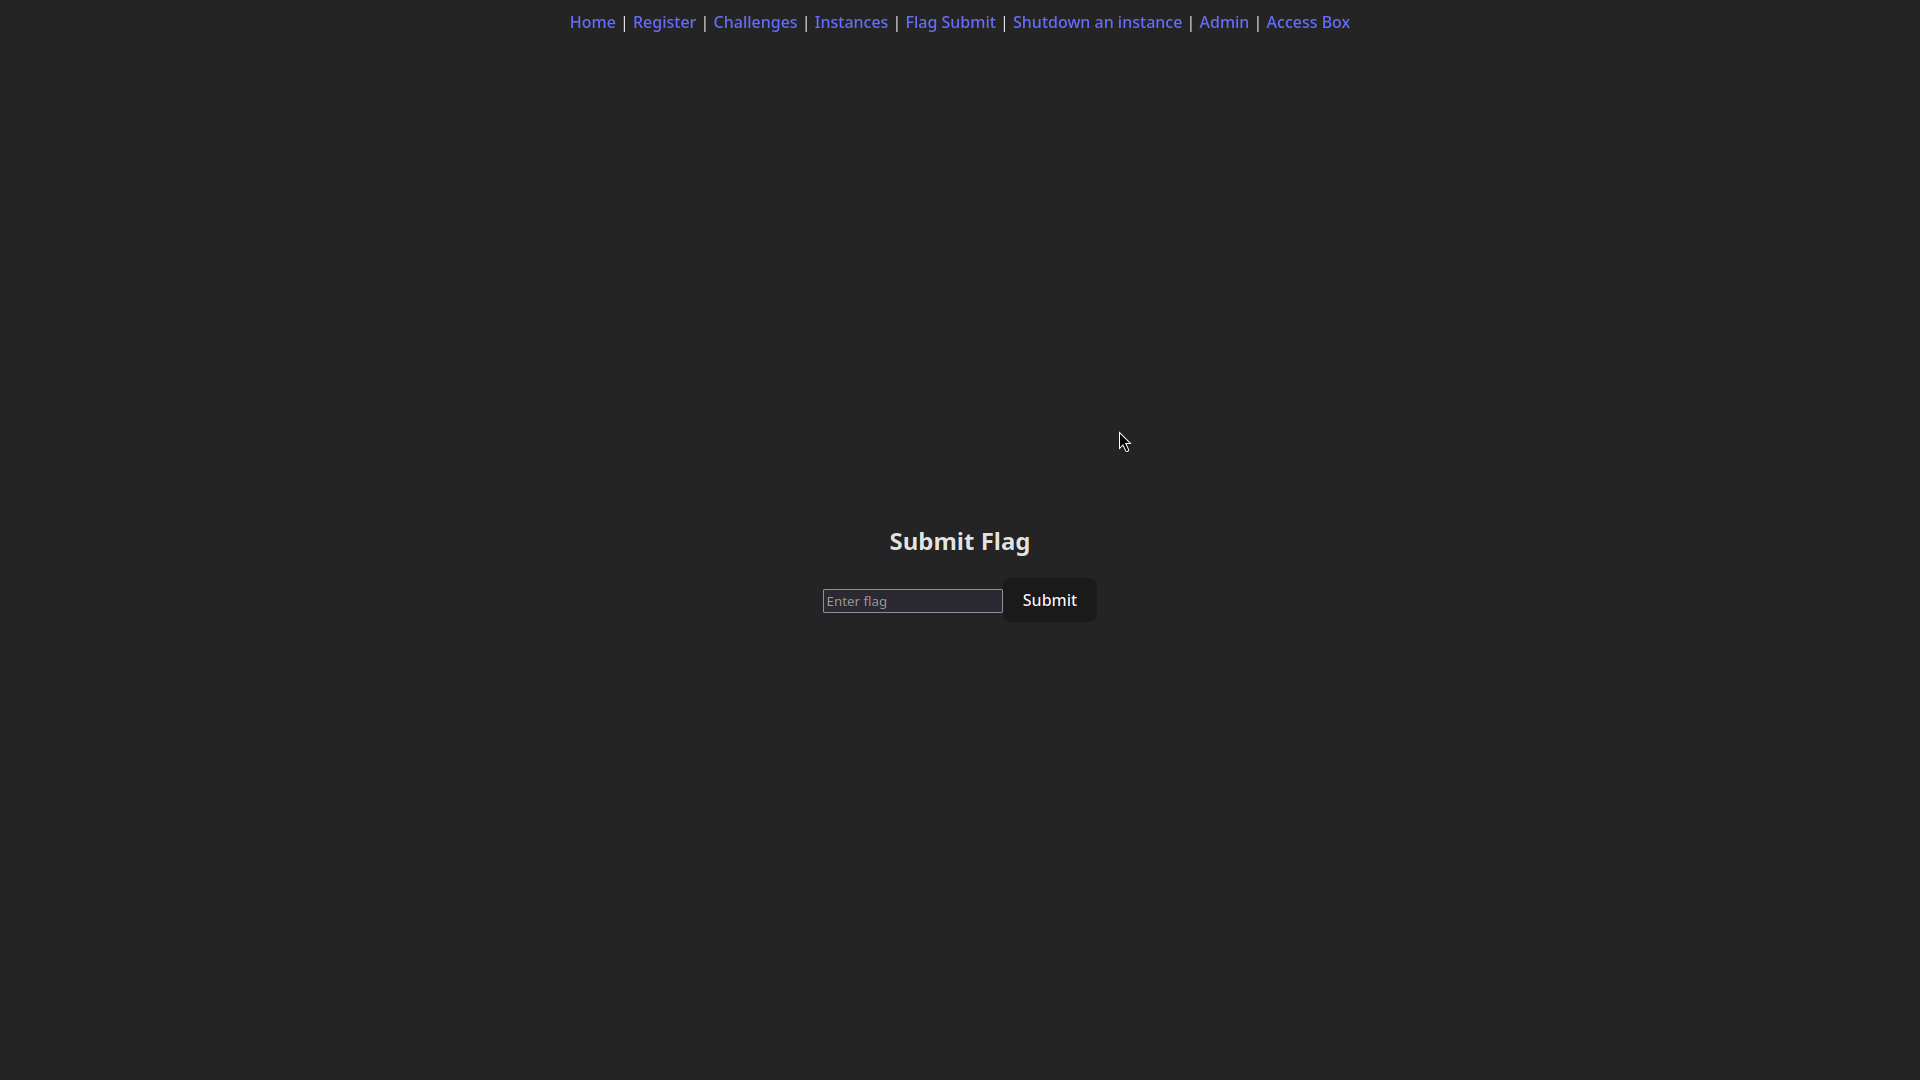
\includegraphics[width=0.8\textwidth]{05-flag.png}
	\caption{Odevzdání vlajky}
	\label{fig:frontend-flag-submit}
\end{figure}

\section{Shutdown an instance}
Na této stránce je možné vypínat právě běžící úlohy uživatele. Uživatel musí zadat ID úlohy, kterou chce vypnout a po kliknutí na tlačítko "Shutdown" se tato úloha vypne.

\begin{figure}[h]
	\centering
	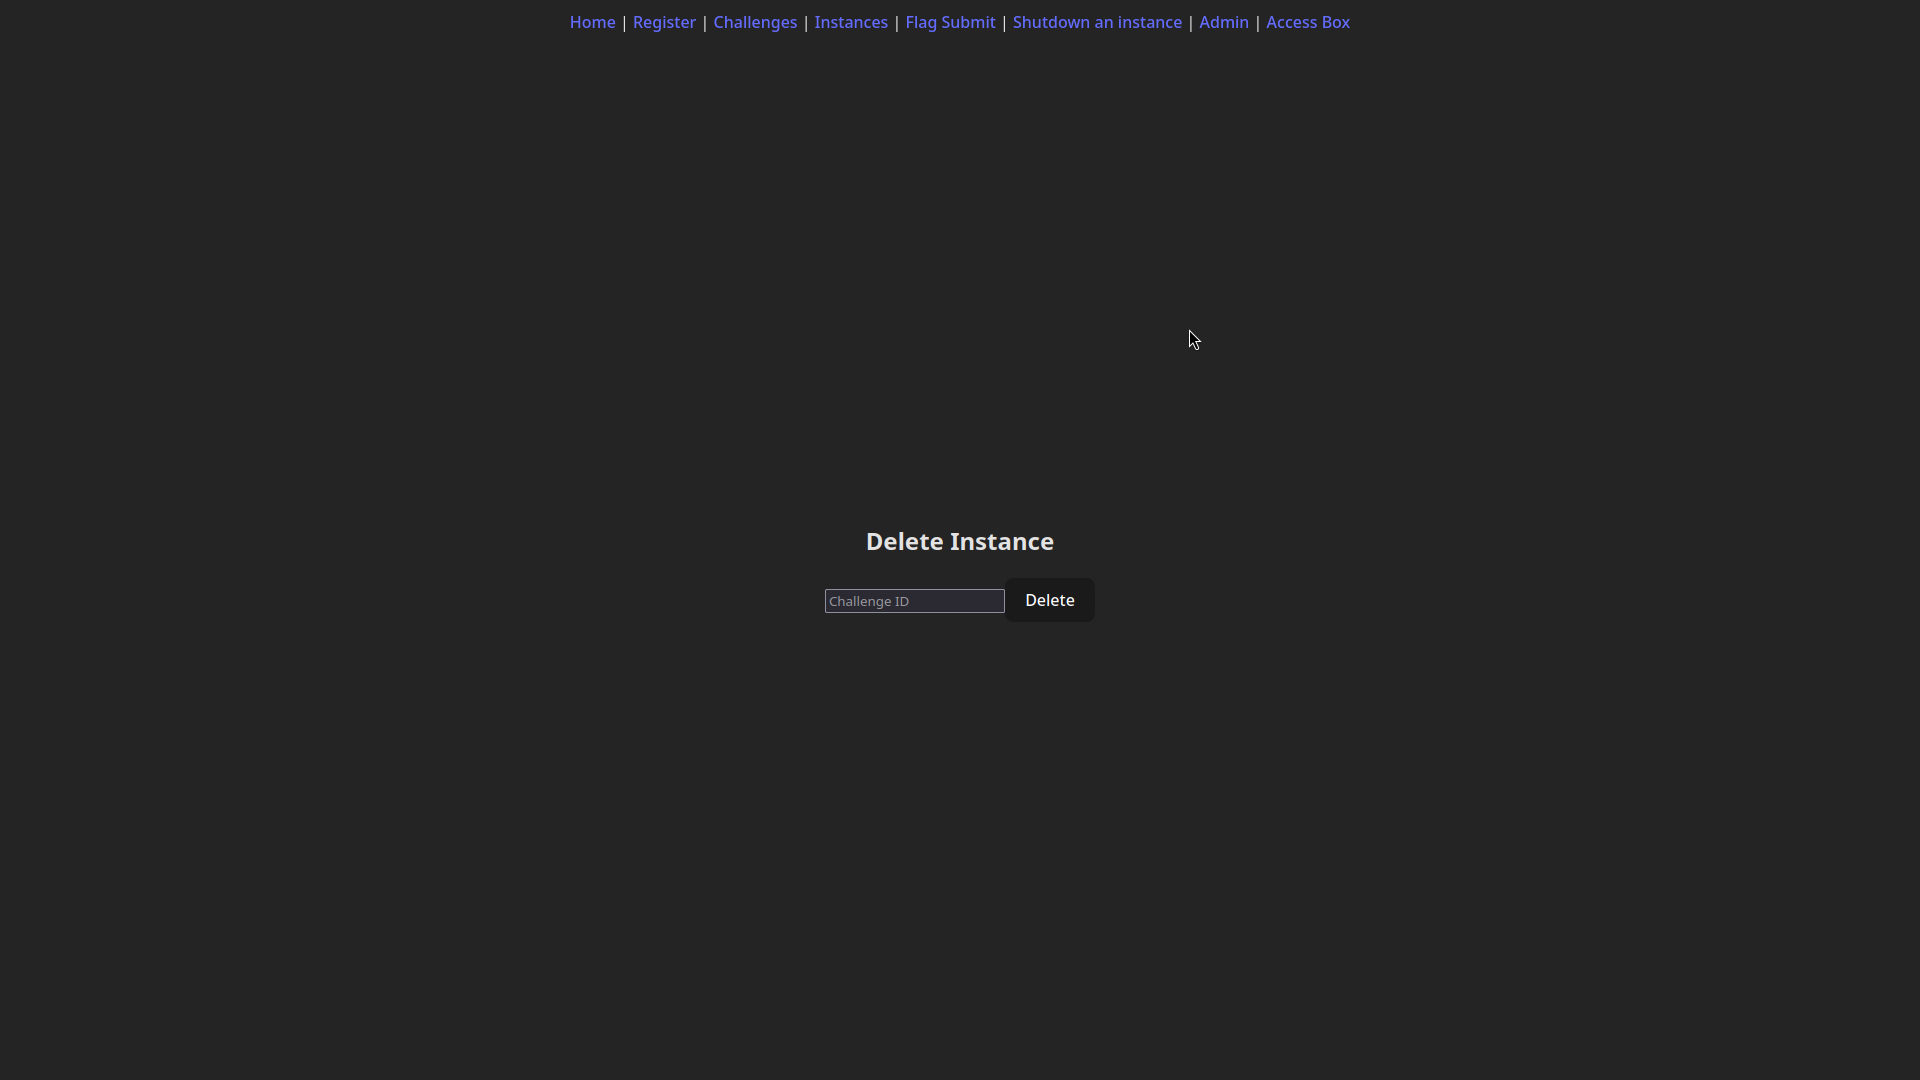
\includegraphics[width=0.8\textwidth]{06-shut.png}
	\caption{Vypnutí úlohy}
	\label{fig:frontend-shutdown}
\end{figure}

\section{Administrátorská sekce}
Sekce pro správce v tuto chvíli obsahuje tři části - vytváření nových úloh, vytváření vlajek, aktualizace uživatelů. Prostředí v administrátorské sekci je děláno tak, aby bylo intuitivní a nebyl problém s tímhle prostředím pracovat. 

Vytváření nových úloh je děláno tak, že je nutné zadat pouze název úlohy, image úlohy a kategorii úlohy - veškeré ostatní části JSON manifestu úlohy jsou generovány na straně serveru automaticky, čímž se minimalizuje prostor na bezpečnostní chyby - není potřeba kontrolovat validitu odevzdaného JSON souboru, ale pouze těchto tří částí. 

Vytváření vlajek pouze požaduje identifikační číslo ulohy, ke které se vlajka váže, a vlajku samotnou.

Aktualizace uživatelů umožňuje změnit uživateli práva nebo změnit heslo uživatele.

Pro bezpečnost této části je využíváno parametru "admin" u JWT tokenu, který je vytvořen při přihlášení uživatele s právy administrátora. Díky tomuto je možné jednoduše ověřit, zda je uživatel oprávněn k použití této části vzhledem k tomu, že s JSON web tokeny nelze manipulovat bez privátního klíče.

\begin{figure}[h]
	\centering
	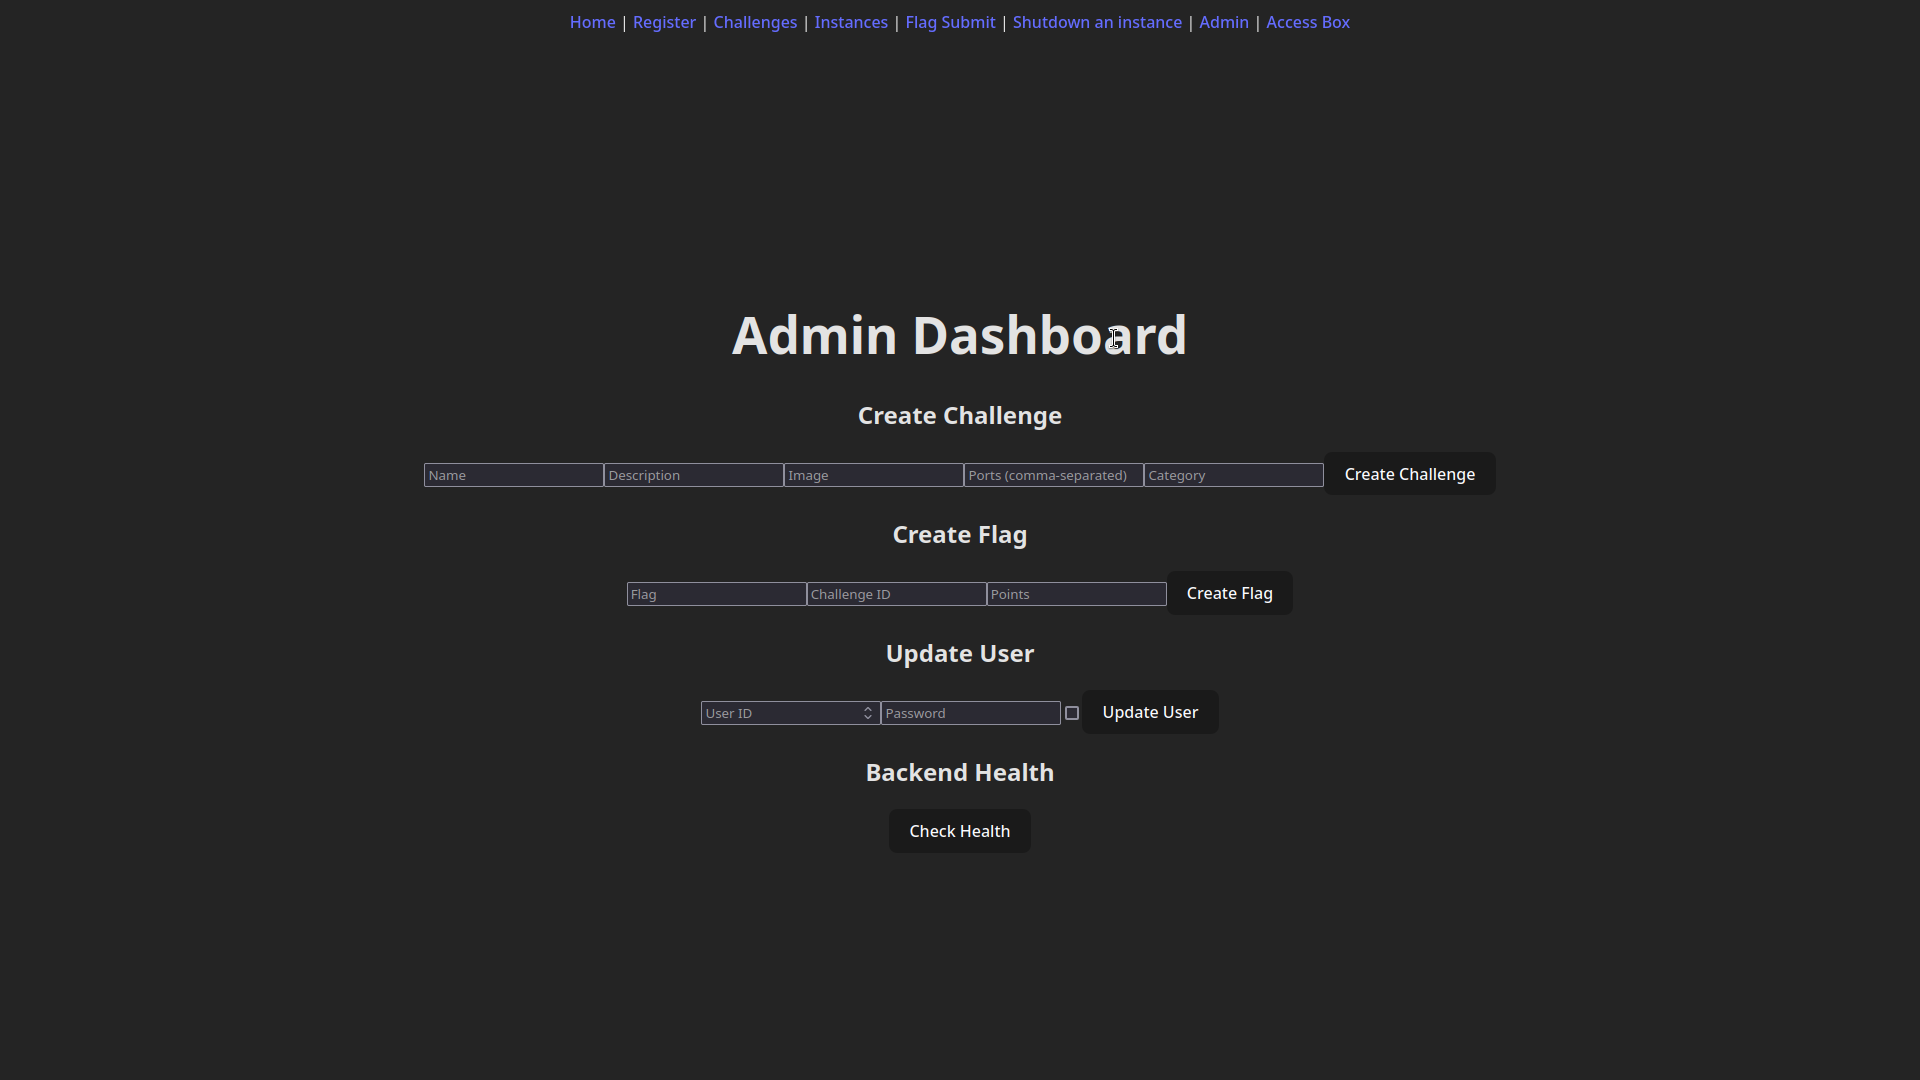
\includegraphics[width=0.8\textwidth]{07-admin.png}
	\caption{Administrátorská sekce}
	\label{fig:frontend-admin}
\end{figure}

\section{Access box}
Jakožto přístup k samotným úlohám je uživateli standardně poskytnut na žádost tzv. Access box, což je kontejner s image kalilinux/kali-last-release, který se nachází ve stejném namespace a tudíž ve stejné síti jakožto úlohy uživatele. 

Toto řešení má oproti řešení pomocí VPN výhodu v tom, že není nutno instalovat žádný software na straně uživatele a není nutno vytvářet certifikáty, popř. uživatele, tudíž je mnohem jednodušší na implementaci a jednodušší na škálování jelikož lze tento kontejner spustit na každém nodu v Kubernetes clusteru.

Použití Kali Linuxu je z důvodu, že je to jedna z nejznámějších distribucí pro pentesting a je také jedna z nejvíce používaných distribucí pro tento účel, což umožňuje uživateli si toto prostředí vyzkoušet.

Ke kontejneru lze přistoupit z webového prostředí, kde lze vidět terminál realizovaný pomocí REST API.
\begin{itemize}
	\item POST /exec
	\item POST /create
	\item GET /logs
	\item GET /health
\end{itemize}
kde první endpoint slouží k odeslání příkazu do kontejneru, druhý k vytvoření nového kontejneru, třetí k získání logů z kontejneru a čtvrtý k zjištění stavu služby.

\begin{figure}[h]
	\centering
	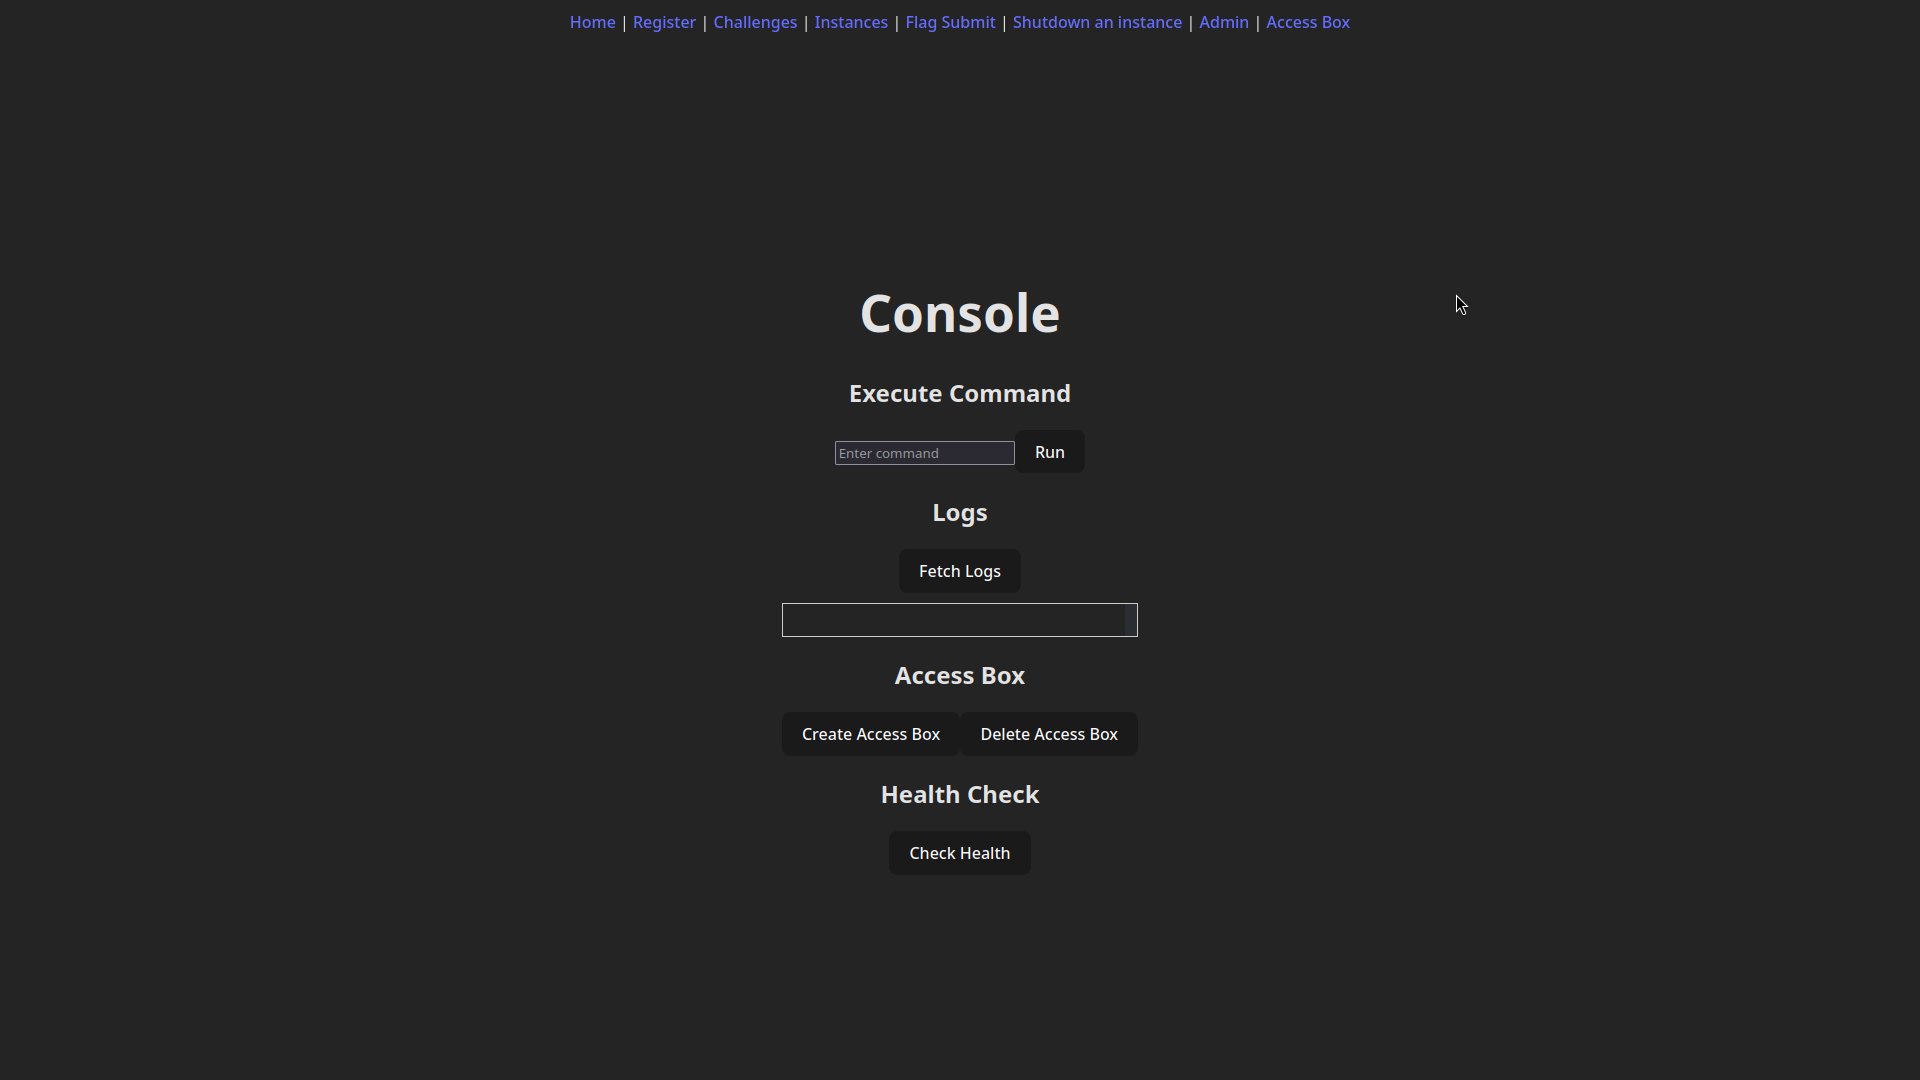
\includegraphics[width=0.8\textwidth]{08-access.png}
	\caption{Access box}
	\label{fig:frontend-access}
\end{figure}

\begin{figure}[h]
	\centering
	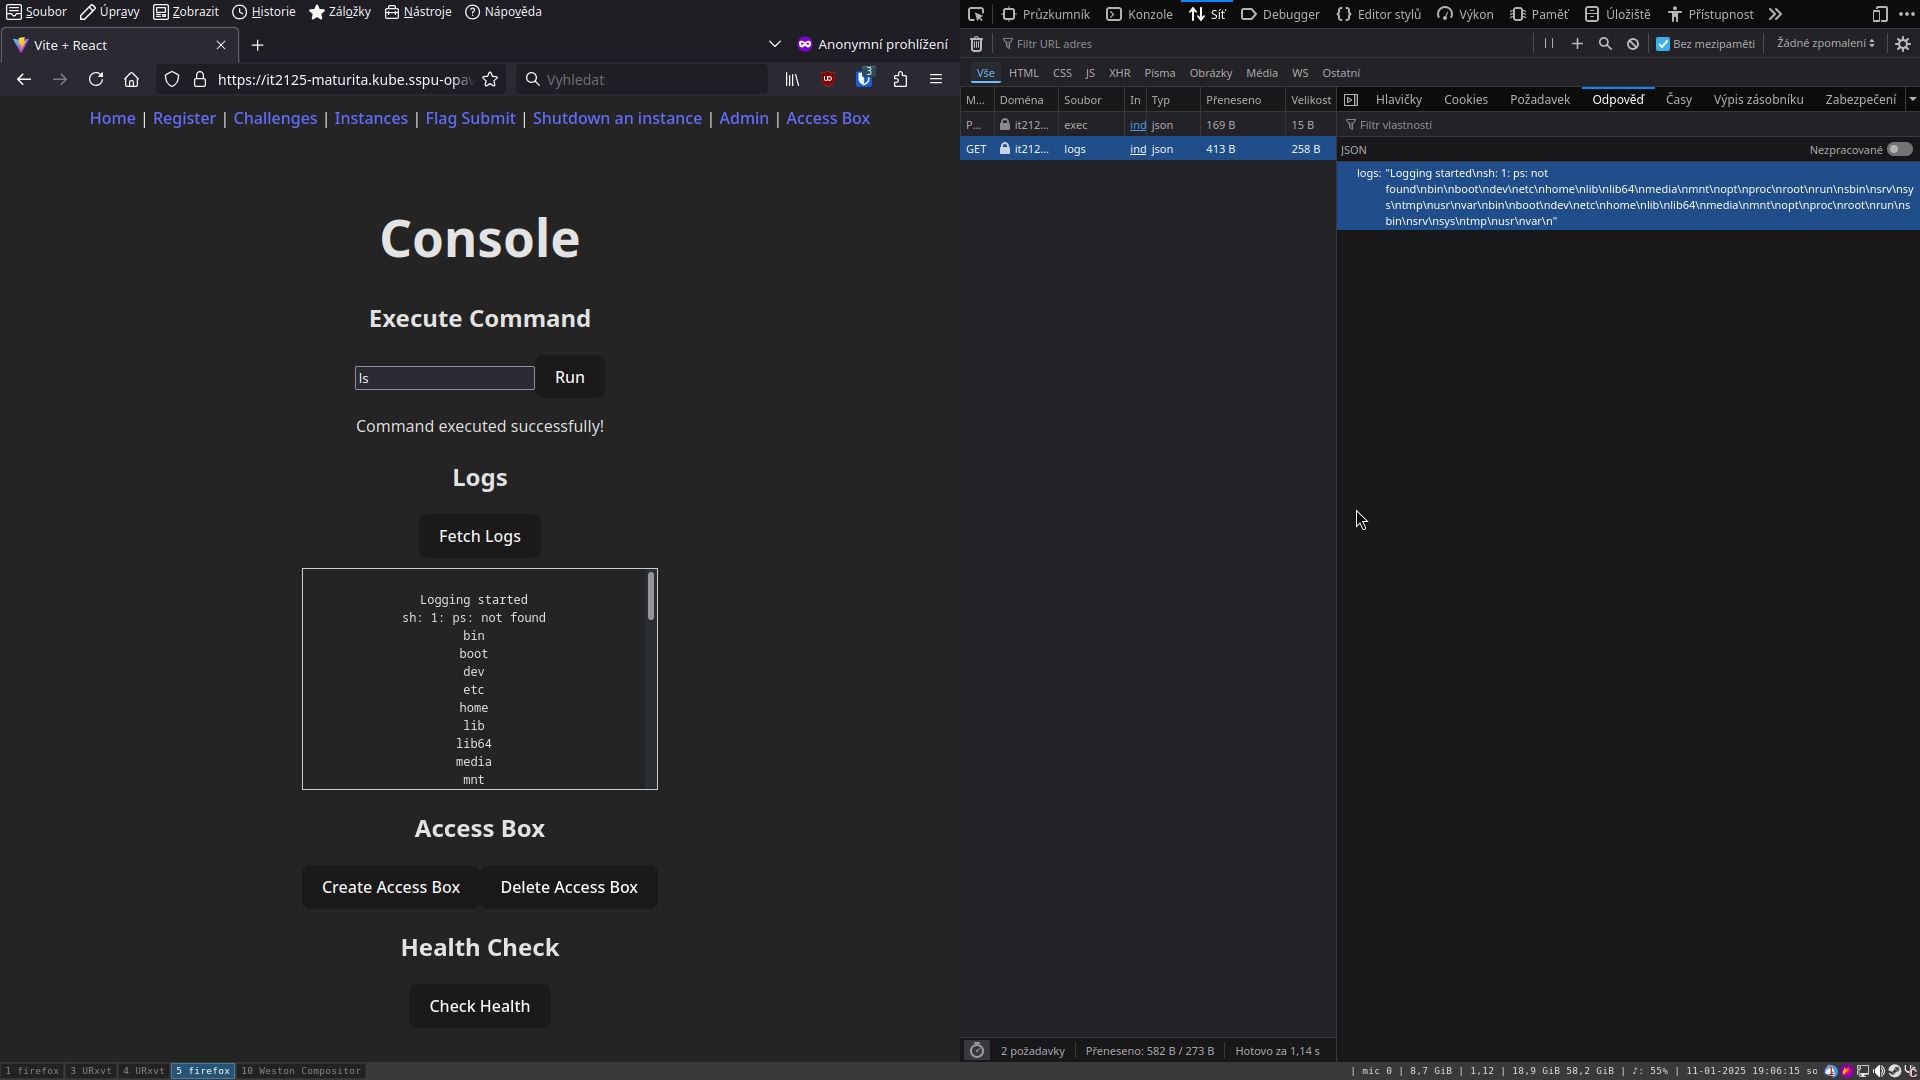
\includegraphics[width=0.8\textwidth]{09-command.png}
	\caption{Odeslání příkazu a logy}
	\label{fig:frontend-command}
\end{figure}

	\chapter{Závěr}

	Celkově bych řekl, že se mi podařilo splnit veškeré cíle, které jsem si stanovil na začátku tohoto projektu. Vytvořil jsem funkční systém pro vytváření a správu úloh CTF typu v systému Kubernetes, který je dostupný na školní síti a je dostatečně zabezpečený. Zároveň jsem se naučil pracovat s mikroslužbami a s prostředím Kubernetes, což byly mé hlavní cíle tohoto projektu.

	V budoucnu bych chtěl do aplikace přidat možnost vytváření vlastních API tokenů, rozšířit frontend a zjednodušit administraci systému pro uživatele. Zároveň bych chtěl do aplikace přidat žebříček uživatelů, možnost vytváření týmů a možnost dynamického skórování vlajek, jako to poskytuje např. systém CTFd.

	Zároveň mi tato aplikace v budoucnu může posloužit jako základ pro další projekty, kde by bylo potřeba vytvářet a spravovat úlohy CTF typu a naučila mě jak pracovat v prostředí s nízkými opravněními i přes projekt na první projekt vyžadující práva vyšší.

	Zdrojový kód tohoto projektu je dostupný na mé GitHub stránce na adrese \url{https://github.com/orgs/jan1s2-maturita/repositories}.
	
	%% literatura
	\renewcommand{\bibname}{Seznam použitých zdrojů}
	\begin{thebibliography}{99}
		\bibitem FFastAPI \textit{FastAPI documentation} [online]. [cit. 2024-12-29]. Dostupné z: https://fastapi.tiangolo.com/
		\bibitem KKubernetes \textit{Kubernetes documentation} [online]. [cit. 2024-12-31]. Dostupné z: https://kubernetes.io/
		\bibitem CCTFd \textit{CTFd project - inspiration} [online]. [cit. 2024-11-21]. Dostupné z: https://ctfd.io/
	\end{thebibliography}
	
	%%% obrázky 
	%\listoffigures
	
	%%% tabulky
	%\listoftables
	
	\appendix %% začínají přílohy
	
	\titleformat{\chapter}[block]{\scshape\bfseries\LARGE}{Příloha \thechapter}{10pt}{\vspace{0pt}}[\vspace{-22pt}] %% nastavení nadpisu u příloh
	
	
	%\chapter{%Příloha A 
		%Spot diagramy a další }
	
	
\end{document}
